%%%%%%%%%%%%%%%%%%%%%%%%%%%%%%%%%%%%%%%%%%%%%%%%%%%%%%%%%%%%%%%%%%%%%%%%%%%%%%%%%%%%%%%%%%%%%%%%%%%%%%
%
%   Filename    : abstract.tex 
%
%   Description : This file will contain your abstract.
%                 
%%%%%%%%%%%%%%%%%%%%%%%%%%%%%%%%%%%%%%%%%%%%%%%%%%%%%%%%%%%%%%%%%%%%%%%%%%%%%%%%%%%%%%%%%%%%%%%%%%%%%%

\chapter{Results and Discussion}
\label{sec:results }

\section{Results Overview}
\label{sec:resultoverview}
In this chapter, the data gathered from the pre-tests, game test, and post-tests are gathered in order to see the effect of Conic Lab in helping player-learners perform better on Precalculus Conic Sections. 

%%%%%%%%%%%%%%%%%%%%%%%%%%%%%%%%%%%%%%%%%%%%%%%%%%%%%%%%%%%%%%%%%%%%%%%%%%%%%%%%%%%%%%%%%%%%%%%%%%%%%%
\begin{comment}
% Conic Lab Pre-test and Post Test
A pre-test was given to the participants before they were allowed to test the game. This was done in order to determine the participant's baseline knowledge about the topic of Precalculus conic sections. There were a total of 12 participants, which are all senior high school students from STEM strand and had a prior experience with learning about the target Precalculus topic for the game. These students range from grade 11 and grade 12. The participants were asked to take the pre-test before testing the game, which would be followed by a post-test after in order to compare their two scores with each other.

The conic test was divided to the four types of conic sections: circle, parabola, ellipse, and hyperbola. The goal is to determine their level of understanding for each of them. Each type of the conic sections have multiple problems about them with varying difficulty.

% MEEGA / Player Opinion
% - Notable trend on the player opinion survey
% Behavioral Analysis 
% - Notable behavior of the participants
% No need for performance testing
\end{comment}
%%%%%%%%%%%%%%%%%%%%%%%%%%%%%%%%%%%%%%%%%%%%%%%%%%%%%%%%%%%%%%%%%%%%%%%%%%%%%%%%%%%%%%%%%%%%%%%%%%%%%%
\subsection{Pre-test and Post-test Results}
Before performing the statistical analysis on the pre-test and post-test data, a test of Normality, the Shapiro-Wilk test, is performed to check the Normality of the data by the difference between the pre-test and post-test with an $\alpha$ = 0.05. The Normality test is done due to the number of participants n = 14. Test results show a p-value = 0.24 $>$ $\alpha$ = 0.05, showing that the data has no significant departure from normality, and we can proceed with a parametric test, a Paired T-Test.

\begin{table}[h]
	\centering
	\caption{Test of Normality (Shapiro-Wilk)}
	\label{tab:testOfNormality(Shapiro-Wilk)}
	{
		\begin{tabular}{lrrrr}
			\toprule
			 &  &  & W & p  \\
			\cmidrule[0.4pt]{1-5}
			Pre-test & - & Post-test & $0.919$ & $0.240$  \\
			\bottomrule
			% \addlinespace[1ex]
			% \multicolumn{5}{p{0.5\linewidth}}{\textit{Note.} Significant results suggest a deviation from normality.} \\
		\end{tabular}
	}
\end{table}

For this study the following are the null hypothesis and the alternative hypothesis:


\begin{tabular}{p{13cm} @{\hspace{1cm}} p{12cm}} 
\textbf{H0:}There is no significant difference between the mean scores of the pre-test and post-test \\ \\
\textbf{H1:}There is significant difference between the mean scores of the pre-test and post-test
\end{tabular}

Given the null and alternative hypotheses, to assess if there was a significant change between the participants’ pre-test and post-test scores, a One-Tailed Paired T-test and a Wilcoxon Signed-Rank test were performed on the data using $\alpha$ = 0.05. Table~\ref{tab:pairedSamplesT-Test} presents the summarized results for the Paired T-Test and Wilcoxon Signed-Rank Test. 



\begin{table}[h]
	\centering
	\caption{Paired Samples T-Test \& Wilcoxon Signed-Rank Test Results}
	\label{tab:pairedSamplesT-Test}
	{
		\begin{tabular}{lrrrrrrr}
			\toprule
			Measure 1 &  & Measure 2 & Test & Statistic & z & df & p  \\
			\cmidrule[0.4pt]{1-8}
			Pre-test & - & Post-test & Student & $-4.189$ & $$ & $12$ & .00063  \\
			$$ & $$ & $$ & Wilcoxon & $0.000$ & $-2.934$ & $$ & $0.002$  \\
			\bottomrule
			% \addlinespace[1ex]
			% \multicolumn{8}{p{0.5\linewidth}}{\textit{Note.} For all tests, the alternative hypothesis specifies that Pretest is less than Posttest.} \\
		\end{tabular}
	}
\end{table}
As shown in table~\ref{tab:pairedSamplesT-Test}, the T-Test's p-value = 0.00063 is less than $\alpha$ = 0.05, suggesting that the difference between the pre-test and post-scores is significant. To further support the t-test observation, the Wilcoxon Signed-Rank test shows a W Statistic of 0, and with $\alpha$ = 0.05 and a sample size of 11 as those whose scores had no difference for both tests were not included, the Critical Value is 10. With the W = 0 $<$ Critical Value = 10, and the shown p-value = 0.002 $<$  $\alpha$ = 0.05, this test also suggests a significant difference in scores between the pre-test and post-test. With the results of both tests, there is substantial evidence to reject the null hylpothesis and say that there is a change in participants' scores after playing the game.

\iffalse
\clearpage
\begin{table}[h]
\hspace*{-1cm}
\begin{tabular}{|c|c|c|c|c|c|c|c|c|}
\hline
$n$ & Pretest & Posttest & Difference & Sign & Absolute Difference & Rank & Rank - & Rank + \\
\hline
1 & 5.00 & 6.00 & -1.00 & -1 & 1 & 1 & 1 & \\
2 & 12.00 & 14.00 & -2.00 & -1 & 2 & 3 & 3 & \\
3 & 7.00 & 13.00 & -6.00 & -1 & 6 & 8.5 & 8.5 & \\
4 & 9.00 & 13.00 & -4.00 & -1 & 4 & 6.5 & 6.5 & \\
5 & 7.00 & 13.00 & -6.00 & -1 & 6 & 8.5 & 8.5 & \\
6 & 9.00 & 9.00 & 0.00 & 0 & - & - & & \\
7 & 5.00 & 7.00 & -2.00 & -1 & 2 & 3 & 3& \\
8 & 2.00 & 2.00 & 0.00 & 0 & - & - & & \\
9 & 11.00 & 13.00 & -2.00 & -1 & 2 & 3 & 3 & \\
10 & 10.00 & 13.00 & -3.00 & -1 & 3 & 5 & 5 & \\
11 & 4.00 & 12.00 & -8.00 & -1 & 8 & 10 & 10 & \\
12 & 6.00 & 10.00 & -4.00 & -1 & 4 & 6.5 & 6.5 & \\
13 & 3.00 & 14.00 & -11.00 & -1 & 11 & 11 & 11 & \\
\hline
 & & & & & & Total & 66(W-) & 0(W+) \\
\hline
\end{tabular}
\caption{Full Wilcoxon Signed-Rank Test}
\label{tab:pretest_posttest_comparison}
\end{table}
\fi


\subsection{MEEGA+ Results}
Particiants' responses for the MEEGA survey are represented as follows.

\begin{center}

\begin{tabular}{|c|c|}
\hline
\textbf{Response} & \textbf{Value} \\
\hline
Strongly Agree & 2 \\
\hline
Agree & 1 \\
\hline
Neutral & 0 \\
\hline
Disagree & -1 \\
\hline
Strongly Disagree & -2 \\
\hline
\end{tabular}
\captionof{table}{Response Values Table}
\end{center}

The averaged scores for the ratings of the participants for each quality factor are positive. The higher scoring quality factors include the games design and the pacing of new challenges both scoring 1.84, the games ability to provide a satisfying feeling of accomplishment with a score of 1.76, and how fun the player had with a score of 1.69. On the other hand, the lower scoring quality factors include, the level of immersion/engagement the player had scoring 0.92, how relevant the game content is to the players interests with 0.84, and the players preference to use the game to learn the material scoring 0.53. \\

To classify the game's quality level, the participants responses are use and to be compared to the criteria as shown in Figure~\ref{fig:MeegaCriteria}. The average of all scores is computed as $\theta$=1.27. $\theta$ is then transformed by a scale of (50,15) with the formula $\theta_{50,15}=50+15* \theta_{1.27}$ resulting in a value of 69.15. This value classifies our game as excellent quality given that $\theta >=$ 65.

\begin{figure}[h]
\hspace*{-1cm}
   \centering                  
   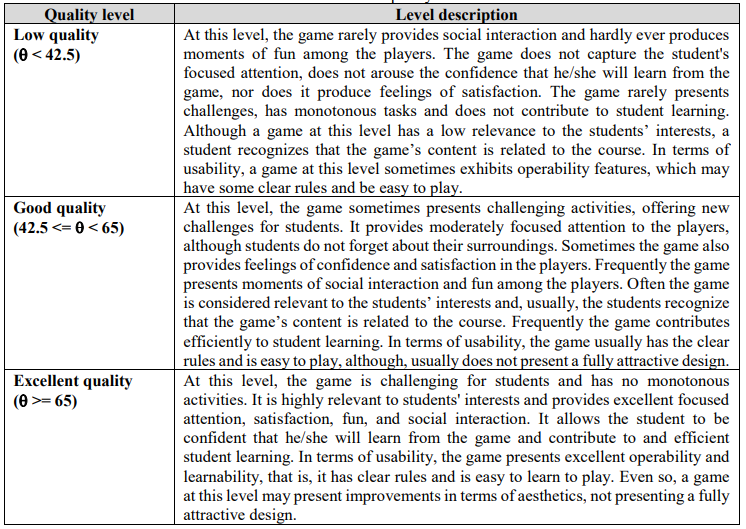
\includegraphics[width=300px,height=200px]{Chapter6/MeegaCriteria.png}      
   \caption{Meega Criteria for Game Quality Classification}
    \label{fig:MeegaCriteria}
\end{figure}
\section{Discussion}

\subsection{Pre-Test and Post-Test Data}
The statistical analysis showed a significant improvement in participants' scores from the pre-test to the post-test, suggesting the game's effectiveness in teaching/improving the participant's understanding of the conic sections. Pre-test scores showed no noticeable patterns in which questions were answered correctly. However, post-test scores indicated a higher likelihood of participants answering correctly in questions involving circles and parabolas and less so for questions involving ellipses and hyperbolas. In terms of improvement, participants improved the most in answering questions that asked them to identify the equation of the conic given specific details of the shape or vice versa.


\subsection{Meega+ Discussion}
Based on the MEEGA results, there were several factors of the game that were positively evaluated by the participants. Specifically, these aspects have scored notably high: game design, pacing of challenges, and overall fun factor. These elements are crucial as they directly contribute to player enjoyment and satisfaction. On the other hand, there were also low scores on some aspects. Specifically, these are the immersion/engagement, relevance to player interests, and educational value aspects.

The game is categorized as "excellent" by the computed average score. This ranking emphasizes the game's capacity to provide enjoyable gameplay and an immersive experience. There is room for development, nevertheless, as evidenced by the lower ratings for immersion, relevance to player interests, and instructional value. In order to improve player engagement and better match the game with player preferences and educational goals, future versions may concentrate on improving these features. The game can be made even better and more efficient by taking care of these issues.



